\documentclass[fullpage]{article}
	\addtolength{\oddsidemargin}{-.875in}
	\addtolength{\evensidemargin}{-.875in}
	\addtolength{\textwidth}{1.75in}

	\addtolength{\topmargin}{-.875in}
	\addtolength{\textheight}{1.75in}

\makeatletter
\setlength{\@fptop}{0pt}
\makeatother
\usepackage[utf8]{inputenc}
\usepackage[pdftex]{graphicx}
\usepackage{mathtools}

\title{\textbf{Computational Robotics} \\ \large Lab 1 - Markov Decision Processes}
\author{Andrew Choi}
\date{October 2019}

\begin{document}
\maketitle

\section{Introduction}

This goal of this lab is to explore finite Markov Decision Processes (MDPs) to control a simple discretized robot. To do so, a gridworld is constructed with well-defined boundaries and rewards. In this gridworld, we develop and implement a model for robot behavior and use it to accomplish a prescribed task.

\section{Mathematical Formulation}

Before delving into the details of the experiment, the finite Markov Decision Process as well as the methods employed (value iteration and policy iteration) are described mathematically.

Markov decision processes (MDPs from hereon) are a classical formalization of sequential decision making. Driven by rewards, these decisions are made not just influenced by immediate rewards, but also by possible future rewards.

The finite MDP can be formulated as a set of states, actions, and rewards.

\section{Experimental Setup}

\subsection{Robot Description}

For the experiment, a simple robot is is considered that will reside in the gridworld and attempt to reach a prescribed goal state. The robot will occupy one grid in the gridworld at any given time and can face any of the twelve headings identified by the hours on a clock $h \in \{0...11\}$. Each action is characterized by moving forward, backward, or staying still. This is followed by a rotation of -1, 0, or 1. From this it can be seen that the action of the robot can be described as a tuple
\[
(a, b),
\]
where $a$ is the movement value and $b$ is the rotation value.
The following restrictions are also applied to the robot's actions:
\begin{enumerate}
\item Attempting to move off the grid results in no linear movement, but the rotation portion will still happen.
\item Aside from restriction 1, the robot can only rotate if it also moves forwards or backwards.
\item If the robot chooses to move "forwards" or "backwards" a pre-rotation error will occur with probability $p_e$
\begin{enumerate}
\item With probability $p_e$ each, robot will first rotate by +1 or -1 before it moves. No pre-rotate with probability $1-p_e$.
\item Choosing to stay still will not incur an error rotation.
\end{enumerate}
\end{enumerate}

Then, it can be seen that the robot is defined by the following discrete action space.
\[
(1, 0), (1, 1), (1,-1), (0,0), (-1,0), (-1,1), (-1,1)
             N_e = 7
\]

\subsection{Created Gridworld and Rewards}
To allow for trajectory simulation, an 8x8 gridworld is constructed. Provided for us are the defined rewards for the states of the gridworld as shown in figure 1.

\begin{figure}[t!]
\centering
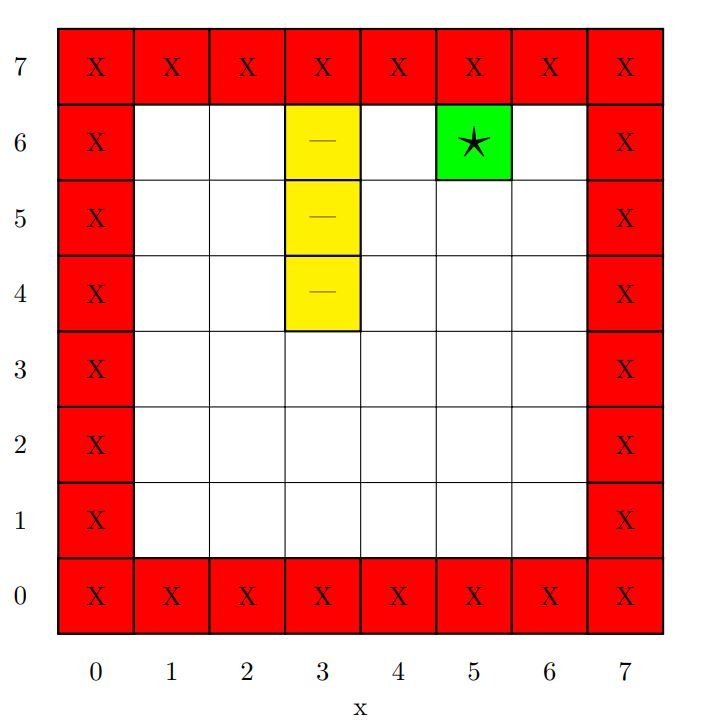
\includegraphics{images/gridworld.jpg}
\caption{Gridworld with set Rewards}
\label{fig:gridworld}
\end{figure}

As the rewards for each state are independent of heading angle, they can be represented graphically on a 2D grid image. As shown above, the boundary states (red and marked X) have a reward of -100. The lane markers 

\subsection{Benchmark}
To be able to properly analyze the benefits provided by following an optimal policy, we first must set a benchmark. This benchmark will be the trajectory generated by a hand-engineered initial policy $\pi_0$. This policy crudely gets to the goal state by simply prioritizing closing the x distance and then the y distance without any regard for rewards \textit{(code in utils.py)}. The plotted trajectory can be seen in figure 2.

\subsection{Scenarios}
With the following setup, we will explore 3 different scenarios:
\begin{enumerate}
\item Reward at goal state independent of heading, $p_e = 0\%$
\item Reward at goal state independent of heading, $p_e=25\%$
\item Reward at goal state +1 only when robot is pointing down $h=6$, $p_e=0\%$
\item Reward at goal state +1 only when robot is pointing down $h=6$, $p_e=25\%$
\end{enumerate}

\section{Experimental Results}

As discussed in the section 1, we employ dynamic programming to find the optimal value function of this MDP. First, we employ policy iteration.

\subsection{Policy Iteration}

First, we define our initial policy $\pi_0$ as the initial policy discussed in section 2.2, initial state $s_0$ as $x = 1, y = 6, h = 6$ (i.e top left corner, pointing down), and error probability $p_e = 0$. Using a discount factor $\gamma = 0.9$, we get the following trajectory.

\subsection{Value Iteration}

For value iteration, we first set the initial value function $V(s) = 0\; \forall s \in S$.

\subsection{Comparisons}
First, 


\section{Conclusion}


\end{document}